%% This is the ctufit-thesis example file. It is used to produce theses
%% for submission to Czech Technical University, Faculty of Information Technology.
%%
%% Get the newest version from
%% https://gitlab.fit.cvut.cz/theses-templates/FITthesis-LaTeX
%%
%%
%% Copyright 2021, Eliska Sestakova and Ondrej Guth
%%
%% This work may be distributed and/or modified under the
%% conditions of the LaTeX Project Public Licenese, either version 1.3
%% of this license or (at your option) any later version.
%% The latest version of this license is in
%%  https://www.latex-project.org/lppl.txt
%% and version 1.3 or later is part of all distributions of LaTeX
%% version 2005/12/01 or later.
%%
%% This work has the LPPL maintenance status `maintained'.
%%
%% The current maintainer of this work is Ondrej Guth.
%% Contact ondrej.guth@fit.cvut.cz for bug reports.
%% Alternatively, submit bug reports into the tracker at
%% https://gitlab.fit.cvut.cz/theses-templates/FITthesis-LaTeX/issues
%%
%%

%%%%%%%%%%%%%%%%%%%%%%%%%%%%%%%%%%%%%%%%%
% CLASS OPTIONS
% language: czech/english/slovak
% thesis type: bachelor/master/dissertation
%%%%%%%%%%%%%%%%%%%%%%%%%%%%%%%%%%%%%%%%%
\documentclass[english,master,unicode]{ctufit-thesis}

%%%%%%%%%%%%%%%%%%%%%%%%%%%%%%%%%%
% FILL IN THIS INFORMATION
%%%%%%%%%%%%%%%%%%%%%%%%%%%%%%%%%%
\ctufittitle{P4 Language Server} % replace with the title of your thesis
\ctufitauthorfull{Bc. Ondřej Kvapil} % replace with your full name (first name(s) and then family name(s) / surname(s)) including academic degrees
\ctufitauthorsurnames{Kvapil} % replace with your surname(s) / family name(s)
\ctufitauthorgivennames{Ondřej} % replace with your first name(s) / given name(s)
\ctufitsupervisor{Ing.\,Viktor Puš,\,Ph.D.\,MBA} % replace with name of your supervisor/advisor (include academic degrees)
\ctufitdepartment{Katedra teoretické informatiky} % replace with the department of your defence
\ctufityear{2023} % replace with the year of your defence
\ctufitdeclarationplace{Prague} % replace with the place where you sign the declaration
\ctufitdeclarationdate{\DTMdisplaydate{2023}{5}{4}{0}} % replace with the date of signature of the declaration

\ctufitabstractCZE{Jazyk P4 je používán pro konfiguraci programovatelných
síťových procesorů. Navzdory své popularitě v odvětví Software Defined
Networking ale zaostává co se podpory programátora týče. V této práci navrhujeme
a implementujeme language server pro jazyk P4, který poskytuje podporu pro
lexikální analýzu, preprocessing a syntaktickou analýzu. Na těchto základech
stavíme automatické doplňování, reporting chyb a navigaci ve zdrojovém kódu.
Language server je implementován v jazyce Rust a integrován do vývojového
prostředí Visual Studio Code.}

\ctufitabstractENG{The P4 language is used for configuring programmable network
processors. Despite its popularity in the Software Defined Networking field, it
suffers from a lack of modern developer tooling. In this thesis, we design and
implement a language server for the P4 language, which provides support for
lexical analysis, preprocessing, and parsing. On these foundations, we build
support for autocompletion, error reporting, and navigation in the source code.
The language server is implemented in the Rust language and integrated into the
Visual Studio Code development environment.}

\ctufitkeywordsCZE{language server protocol, language server, syntaktická analýza, sémantická analýza, P4, SDN, vývojářské nástroje}
\ctufitkeywordsENG{language server protocol, language server, parsing, semantic analysis, P4, SDN, developer tools}
%%%%%%%%%%%%%%%%%%%%%%%%%%%%%%%%%%
% END FILL IN
%%%%%%%%%%%%%%%%%%%%%%%%%%%%%%%%%%

%%%%%%%%%%%%%%%%%%%%%%%%%%%%%%%%%%
% CUSTOMIZATION of this template
% Skip this part or alter it if you know what you are doing.
%%%%%%%%%%%%%%%%%%%%%%%%%%%%%%%%%%

\RequirePackage{iftex}[2020/03/06]
\iftutex % XeLaTeX and LuaLaTeX
    \RequirePackage{ellipsis}[2020/05/22] %ellipsis workaround for XeLaTeX
\else
    \RequirePackage[utf8]{inputenc}[2018/08/11] %this file encoding
    \RequirePackage{lmodern}[2009/10/30] % vector flavor of Computer Modern font
\fi

% hyperlinks
\RequirePackage[pdfpagelayout=TwoPageRight,colorlinks=false,allcolors=decoration,pdfborder={0 0 0.1}]{hyperref}[2020-05-15]

% uncomment the following to hide all hyperlinks
% \RequirePackage[pdfpagelayout=TwoPageRight,hidelinks]{hyperref}[2020-05-15]

\RequirePackage{pdfpages}[2020/01/28]

\setcounter{secnumdepth}{4} % numbering sections; 4: subsubsection



%%%%%%%%%%%%%%%%%%%%%%%%%%%%%%%%%%
% CUSTOMIZATION of this template END
%%%%%%%%%%%%%%%%%%%%%%%%%%%%%%%%%%


%%%%%%%%%%%%%%%%%%%%%%
% DEMO CONTENTS SETTINGS
% You may choose to modify this part.
%%%%%%%%%%%%%%%%%%%%%%
\usepackage{dirtree}
\usepackage[style=iso]{datetime2}
\usepackage{fnpct}
\usepackage{lipsum,tikz}
\usepackage{csquotes}
\usepackage[acronym,nonumberlist,toc,numberedsection=autolabel]{glossaries}
\makeglossaries
\usepackage[colorinlistoftodos,prependcaption,textsize=tiny]{todonotes}
\usepackage[style=iso-numeric]{biblatex}
\addbibresource{text/bib-database.bib}
\usepackage{hyperref}
\usepackage{listings} % typesetting of sources
% \usepackage{minted} % typesetting of sources
\usepackage{multicol}
\usepackage{pdfcomment}
\usepackage{tikz}
\usetikzlibrary{automata,backgrounds,fit,positioning,shapes}
\usepackage{tcolorbox}
% libertine without tt
\usepackage[tt=false]{libertine}
\usepackage[libertine]{newtxmath}

% TODO: this is only for correct typesetting of todonotes
\setlength{\marginparwidth}{3.3cm}

%theorems, definitions, etc.
\theoremstyle{plain}
\newtheorem{theorem}{Theorem}
\newtheorem{lemma}[theorem]{Lemma}
\newtheorem{corollary}[theorem]{Corollary}
\newtheorem{proposition}[theorem]{Proposition}
\newtheorem{definition}[theorem]{Definition}
\theoremstyle{definition}
\newtheorem{example}[theorem]{Example}
\theoremstyle{remark}
\newtheorem{note}[theorem]{Note}
\newtheorem*{note*}{Note}
\newtheorem{remark}[theorem]{Remark}
\newtheorem*{remark*}{Remark}
\numberwithin{theorem}{chapter}
%theorems, definitions, etc. END
%%%%%%%%%%%%%%%%%%%%%%
% DEMO CONTENTS SETTINGS END
%%%%%%%%%%%%%%%%%%%%%%


% locate combining diacritics
\DeclareUnicodeCharacter{0301}{*************************************}

\begin{document}
\frontmatter\frontmatterinit % do not remove these two commands


\includepdf{resources/assignment-include.pdf} % replace that file with your thesis assignment provided by study office

\thispagestyle{empty}\cleardoublepage\maketitle % do not remove these three commands

\imprintpage % do not remove this command

\tableofcontents % do not remove this command
%%%%%%%%%%%%%%%%%%%%%%
% list of other contents: figures, tables, code listings, algorithms, etc.
% add/remove commands accordingly
%%%%%%%%%%%%%%%%%%%%%%
\listoffigures % list of figures
\begingroup
\let\clearpage\relax
\listoftables % list of tables

\endgroup % Moved the \endgroup here because list of listings had heading on one page and the list on the next

\lstlistoflistings % list of source code listings generated by the listings package
% \listoflistings % list of source code listings generated by the minted package
%%%%%%%%%%%%%%%%%%%%%%
% list of other contents END
%%%%%%%%%%%%%%%%%%%%%%

%%%%%%%%%%%%%%%%%%%
% ACKNOWLEDGMENT
% FILL IN / MODIFY
% This is a place to thank people for helping you. It is common to thank your supervisor.
%%%%%%%%%%%%%%%%%%%
\begin{acknowledgmentpage}
	I would like to thank Timothy Roberts and Adam Reynolds for their kindness
	and support of my internship during challenging times at Intel. Thanks to my
	supervisor, Viktor Puš, without whose enthusiasm I would never have applied
	for the internship. And, last but not least, thanks to my family and friends
	for making my life better than I deserve.
\end{acknowledgmentpage}
%%%%%%%%%%%%%%%%%%%
% ACKNOWLEDGMENT END
%%%%%%%%%%%%%%%%%%%


%%%%%%%%%%%%%%%%%%%
% DECLARATION
% FILL IN / MODIFY
%%%%%%%%%%%%%%%%%%%
% INSTRUCTIONS
% ENG: choose one of approved texts of the declaration. DO NOT CREATE YOUR OWN. Find the approved texts at https://courses.fit.cvut.cz/SFE/download/index.html#_documents (document Declaration for FT in English)
% CZE/SLO: Vyberte jedno z fakultou schvalenych prohlaseni. NEVKLADEJTE VLASTNI TEXT. Schvalena prohlaseni najdete zde: https://courses.fit.cvut.cz/SZZ/dokumenty/index.html#_dokumenty (prohlášení do ZP)
\begin{declarationpage}
	I hereby declare that the presented thesis is my own work and that I have
	cited all sources of information in accordance with the Guideline for
	adhering to ethical principles when elaborating an academic final thesis.

	I acknowledge that my thesis is subject to the rights and obligations
	stipulated by the Act No. 121/2000 Coll., the Copyright Act, as amended. In
	accordance with Section 2373(2) of Act No. 89/2012 Coll., the Civil Code, as
	amended, I hereby grant a non-exclusive authorization (licence) to utilize
	this thesis, including all computer programs that are part of it or attached
	to it and all documentation thereof (hereinafter collectively referred to as
	the "Work"), to any and all persons who wish to use the Work. Such persons
	are entitled to use the Work in any manner that does not diminish the value
	of the Work and for any purpose (including use for profit). This
	authorisation is unlimited in time, territory and quantity.
\end{declarationpage}
%%%%%%%%%%%%%%%%%%%
% DECLARATION END
%%%%%%%%%%%%%%%%%%%

\printabstractpage % do not remove this command

%%%%%%%%%%%%%%%%%%%
% SUMMARY
% FILL IN / MODIFY
% OR REMOVE ENTIRELY (upon agreement with your supervisor)
% (appropriate to remove in most theses)
%%%%%%%%%%%%%%%%%%%
\begin{summarypage}
\section*{Introduction}

We open with an overview of the networking setting that led to the development
of the P4 language. After a brief survey of existing tooling, we decide to
implement our own.

\section*{The P4 Language}

Next, we delve into the details of P4 to better understand the commonalities and
differences between it and conventional programming languages.

\section*{Language Server Architecture}

We explore the language server protocol and existing LSP-compliant tools. We
also survey architectural themes in conventional compilers and pluck a few ripe
ideas for our own use later.

\section*{Design}

In this chapter, we detail the design of our language server. We go over the key
abstractions and algorithms, motivating our design decisions along the way.

\section*{Results}

The final chapter closes with lessons learned, our implementation's strengths,
and areas where it falls short. We conclude with a discussion of future work.

\end{summarypage}
%%%%%%%%%%%%%%%%%%%
% SUMMARY END
%%%%%%%%%%%%%%%%%%%

%%%%%%%%%%%%%%%%%%%
% ABBREVIATIONS
% FILL IN / MODIFY
% OR REMOVE ENTIRELY
% List the abbreviations in lexicography order.
%%%%%%%%%%%%%%%%%%%

\printglossaries
%%%%%%%%%%%%%%%%%%%
% ABBREVIATIONS END
%%%%%%%%%%%%%%%%%%%

\mainmatter\mainmatterinit % do not remove these two commands

%%%%%%%%%%%%%%%%%%%
% THE THESIS
% MODIFY ANYTHING BELOW THIS LINE
%%%%%%%%%%%%%%%%%%%

% Do not forget to include Introduction
%---------------------------------------------------------------
% \chapter{Introduction}
% uncomment the following line to create an unnumbered chapter
\chapter*{Introduction}\addcontentsline{toc}{chapter}{Introduction}\markboth{Introduction}{Introduction}
%---------------------------------------------------------------
\setcounter{page}{1}

% acronyms
\newacronym{api}{API}{application programming interface}
\newacronym{asic}{ASIC}{application-specific integrated circuit}
\newacronym{dsl}{DSL}{domain-specific language}
\newacronym{fpga}{FPGA}{field-programmable gate array}
\newacronym{ide}{IDE}{integrated development environment}
\newacronym{lsp}{LSP}{Language Server Protocol}
\newacronym{onf}{ONF}{Open Networking Foundation}
\newacronym{p4}{P4}{Programming Protocol-independent Packet Processors}
\newacronym{repl}{REPL}{read-eval-print loop}
\newacronym{sdn}{SDN}{software-defined networking}
\newacronym{xml}{XML}{eXtensible Markup Language}
\newacronym{yacc}{YACC}{Yet Another Compiler-Compiler}
\newcommand{\pfs}{\texorpdfstring{{P}4\textsubscript{16}}{P4 16} }

% The following environment can be used as a mini-introduction for a chapter.
% Use that any way it pleases you (or comment it out). It can contain, for
% instance, a summary of the chapter. Or, there can be a quotation.
\begin{chapterabstract}
	\todo[inline]{abstract}
\end{chapterabstract}

\acrfull{p4} is a domain-specific language for programming network switches. It
became widely popular in \acrfull{sdn} since its introduction in
2014\cite{p4original}, and has been described as the \emph{natural evolution}
of OpenFlow, a standard communications protocol for \acrshort{sdn}.
\acrshort{p4} lets a network engineer specify the data plane\footnote{Also known
as the ``forwarding plane."} of a router architecture independently of the
underlying hardware. A \acrshort{p4} compiler can then synthesise microcode for
a given switch platform and generate library files for the control plane. Unlike
previous approaches in \acrshort{sdn}, \acrshort{p4} is does not have built-in
support for common network protocols like TCP, IP, or Ethernet. Instead, the
language provides protocol-independent constructs that users can leverage in
order to define arbitrary protocols and instruct a flexible network switch on
how to handle them.

In 2017, \acrshort{p4} underwent a major redesign\cite{p416} which simplified
the syntax and removed special-purpose language constructs in favour of more
general solutions\footnote{Specifically, features like counters and checksum
units were replaced by \texttt{extern}s, a universal construct for specifying
additional hardware capabilities not covered by the core \todo[inline]{word
here?}. The language shrank from over 70 to less than 40
keywords.\cite{p416:v1:spec:comparison}}. The redesigned language is known as
\pfs\cite{p416:v123:spec} and its specification has since received more
incremental updates.

%-------------------------------%
\section*{A Growing Community}
%-------------------------------%

\acrshort{p4} gave rise to a varied ecosystem of commercial offerings of both
hardware and software. It spawned several academic projects that investigated
its semantics\cite{doenges2021petr4}, allocation to heterogeneous
hardware\cite{sultana2021flightplan}, open-source network
testing\cite{antichi2014osnt}, and sketch-based
monitoring\cite{namkung2022sketchlib}, among many
others\cite{liatifis2023advancingp4survey}. The \acrfull{onf}
maintains\cite{p4onf} an open-source reference implementation of a
\pfs\footnote{Although primarily developed for \pfs since the revision of the
language, it is also capable of migrating P4\textsubscript{14} programs to \pfs
or directly compiling them.} compiler frontend and mid\-end, along with several
backends:

\begin{description}
	\item[p4c-bm2-ss] Targets a sample software switch for testing purposes.
	\item[p4c-dpdk] Targets the DPDK software switch (SWX) pipeline\cite{dpdkDPDKRelease}.
	\item[p4c-ebpf] Generates C code which can be compiled to eBPF
		and then loaded in the Linux kernel.
	\item[p4test] A source-to-source P4 translator for testing, learning compiler
		internals and debugging.
	\item[p4c-graphs] Generates visual representations of P4 programs.
	\item[p4c-ubpf] Generates eBPF code that runs in user-space.
	\item[p4tools] A platform for P4 test utilities, includes a test-case
		generator for P4 programs.
\end{description}

All of these components are open source. The frontend and mid\-end of the
reference compiler provide a foundation for hardware vendors to support
\acrshort{p4} in their products and serve the community in resolving
discrepancies between commercial compilers and the language specification.

Despite this growth, \acrshort{p4} has only mediocre support for real-time
feedback to the programmer -- the vast majority of open and commercial tools
rely on compiler output to provide semantic insight into a P4
program\cite{p4insight}, or, as evidenced by the open backends, are parts of the
compiler proper.\todo{make the case for real-time feedback and better error
reporting}

%-----------------------------------------%
\section*{Language Servers to the Rescue}
%-----------------------------------------%

Over the last decade\todo{poor opening? This should be in another section too},
\emph{language servers} became a popular architecture\cite{barros2022editing}
for providing semantically informed editing features in integrated developer
environments and lightweight source code editors alike. Although examples of
language server -like tools predate their standardization\cite{bour2018merlin},
a major milestone in their development was the introduction of the
\acrfull{lsp}. The support of \acrshort{lsp} in Visual Studio Code seeded an
ever-growing environment of cross-platform tooling for a variety of programming,
configuration, specification, and markup languages. Their success can be
attributed in part to the investment by Microsoft. However, \acrshort{lsp} as a
standard has much technical merit.

Before the introduction of a common communication interface between
language-specific tooling and a given source code editor, implementors had to
create and maintain extensions for any number of different environments, often
in several programming languages. For example, take an editor plugin providing
smart completion and "go to definition" features for the Python programming
language. Suppose the author aims to extend Vim, Emacs, and IntelliJ IDEA. They
would therefore have to reimplement the given functionality in vimscript, Emacs
Lisp, and a JVM-based language. Even though recent innovations in classical text
editors\todo{Neovim} have partly moved away from using their own
\acrshort{dsl}'s, the author is still burdened with three times the
implementation work, as every development environment \acrshort{api} is
different.

The solution to this problem is to split editor extensions according to the
client-server model. The major implementation work for domain-specific
functionality resides on the server side, whereas the client is only a
relatively thin wrapper that adapts a given editor's API. Implementors can build
many thin clients for different development environments that all connect to the
same \emph{language server}. \acrshort{lsp}'s raison d'être is support of this
model in Visual Studio Code.

Coden\-vy, Microsoft, and Red Hat collaborated on standardizing the protocol to
enable other tools to benefit from shared
tooling\cite{sdtimesCodenvyMicrosoft,infoworldMicrosoftbackedLanguage}.

% these comments make the section visible from the editor minimap
%-------------------%
%-------------------%
%-------------------%
%-------------------%
%-------------------%
%-------------------%
%-------------------%
%-------------------%
%-------------------%
%-------------------%
%-------------------%
\section{Outline}
%-------------------%
%-------------------%
%-------------------%
%-------------------%
%-------------------%
%-------------------%
%-------------------%
%-------------------%
%-------------------%
%-------------------%
%-------------------%
%-------------------%

\begin{enumerate}
	\item (intro) P4 information
	\item (intro) language servers, VS Code (screenshots, c++?)
	\item design: overview of the architecture, interfaces with the editor, what
		needs to be implemented
	\item subsections about problems that needed solving, but most should go into
		the design part!
	\item results, what it can do, open-source repository, performance metrics
		(aim for interactivity)
	\item conclusion, next steps
\end{enumerate}








\todo[inline]{authorship: link to GitHub, detail which non-critical parts were
implemented by a colleague}


\begin{lstlisting}[
	caption={~Useless code},
	label=list:8-6,
	captionpos=t,
	float,
	abovecaptionskip=-\medskipamount,
	belowcaptionskip=\medskipamount,
	language=C
]
	#include<stdio.h>
	#include<iostream>
	// A comment
	int main(void)
	{
		printf("Hello World\n");
		return 0;
	}
\end{lstlisting}

%%%%%%%%%%%%%%%%%%%%%%%%%%%%%%%%%
% alternative using package minted for source highlighting
% package minted requires execution with `-shell-escape'
% e.g., `xelatex -shell-escape ctufit-thesis.tex'
% \begin{listing}
% \caption{Zbytečný kód}\label{list:8-6}
% \begin{minted}{C}
%     #include<stdio.h>
%     #include<iostream>
%     // A comment
%     int main(void)
%     {
%         printf("Hello World\n");
%         return 0;
%     }
% \end{minted}
% \end{listing}
% %%%%%%%%%%%%%%%%%%%%%%%%%%%%%%%%%

\begin{table}\centering
\caption[Příklad tabulky]{~Typesetting math}\label{tab:mathematics}
\begin{tabular}{l|l|c|c}
	Typ	& Prostředí	&
		\LaTeX{}ovská zkratka	& \TeX{}ovská zkratka	\tabularnewline \hline
	Text	& \verb|math|	&
		\verb|\(...\)|	& \verb|$...$|	\tabularnewline \hline
	Displayed	& \verb|displaymath|	&
		\verb|\[...\]|	& \verb|$$...$$|	\tabularnewline
\end{tabular}
\end{table}


%---------------------------------------------------------------
\chapter{The P4 Language}
%---------------------------------------------------------------

\begin{chapterabstract}
	\dots in which we delve into the syntax and semantics of \acrshort{p4},
	explain its use cases, and discuss the differences to conventional programming
	languages.
\end{chapterabstract}

One of the original motivations behind \acrshort{p4} was the need for
restriction. While other \acrlong{dsl}s, such as Click\todo{citation}, existed
at the time, their embeddings within general-purpose programming languages made
it difficult to analyze data dependencies crucial for scheduling parallel
execution. The expressiveness of a language complicates its efficient
compilation. In the words of Robert Harper,

\begin{displayquote}
	\textit{The expressive power of a programming language arises from its
	strictures and \emph{not} from its affordances.}

	-- Robert Harper, \citedate*{pfpl1oplss2019} \cite{pfpl1oplss2019}
\end{displayquote}

Rather than embedding \acrshort{p4} in an existing language, these
considerations motivated a clean-slate design. However, to understand why is
packet processing any different from tasks suited to general-purpose programming
languages, we need to familiarise ourselves with the switching architecture.

%----------------------------%
\section{What's in a switch}
%----------------------------%

In the following text, we choose to use \emph{switch} to mean a general packet
forwarding device. Examples of switches are

A network switch
\todo[inline]{need a readable description of this \& network routing, also
citations in the text below}

Traditionally, these devices were examples of fixed-function hardware. Various
networking protocols were implemented directly in circuitry, which made them
efficient, but inflexible. It is impossible to reconfigure a fixed-function
\acrshort{asic} to process a protocol it was not explicitly designed for in
advance. If a new, backward-incompatible version of a given protocol emerges, or
if a hardware error is found in the chip, the network administrators need to
perform a costly hardware replacement in order to support, respectively
circumvent it. Moreover, fixed-function hardware design is a lengthy and
resource-intensive process. It may take several years before an updated
fixed-function chip hits the market.

The innovation of recent years is the introduction of \emph{programmable}
network processors, which can change the set of supported protocols on the fly.
These are similar to \acrshort{fpga}s in their reconfigurability, but
specialised to packet switching and routing, which makes them more efficient. A
programmable network switch has typically no prior knowledge of networking
protocols but contains efficient circuitry for parsing and pattern-matching in
order to support arbitrary\footnote{To some degree of complexity supported by
the circuit.} protocols uploaded to the chip as microcode. While programmable
networking hardware does incur a penalty for

Other implementations of packet switching are also common. The already mentioned
\acrlong{fpga}s can be programmed to simulate programmable or fixed-function
networking hardware, and thus allow an even higher degree of flexibility.
Naturally, \acrshort{fpga}s are less efficient than the circuits they simulate.
Finally, there are software switches, programs for widespread processor
architectures and operating systems, such as x86 and Linux. A software switch
represents the peak of flexibility, programmability, and requires no special
hardware other than what is already commonly present in conventional computers.
Purely software-based solutions cannot compete in energy efficiency with any of
the other approaches, but are useful for testing and in small-scale networks.

\begin{figure}[t]
	\includegraphics[
		clip,
		page=3,
		trim=11.5cm 12.3cm 2.7cm 10.3cm, % left bottom right top (insane, I know)
		width=1.00\textwidth
	]{resources/p4original.pdf}
	\caption{The original \acrshort{p4}\textsubscript{14} abstract forwarding
	model\cite{p4original}.}
	\label{fig:abstract-forwarding-model}
\end{figure}

To support network configurations regardless of their physical implementation,
the original \acrshort{p4} paper defines the target-independent \emph{abstract
forwarding model}, outlined in Figure~\ref{fig:abstract-forwarding-model}. This
model assumes an end-to-end pipeline split into \emph{ingress} and \emph{egress}
parts. An arriving packet is first parsed to recognize the headers present
therein. The model assumes that the payload --  is handled separately by the device
and is not available for pattern-matching.

\todo[inline]{finish the model description, mention deparsers, explain metadata}

A lifetime may end early if the packet is dropped during processing. Dropping is
indicated by mutating metadata.

%--------------------------%
\section{The \pfs language}
%--------------------------%

\begin{figure}[t]
	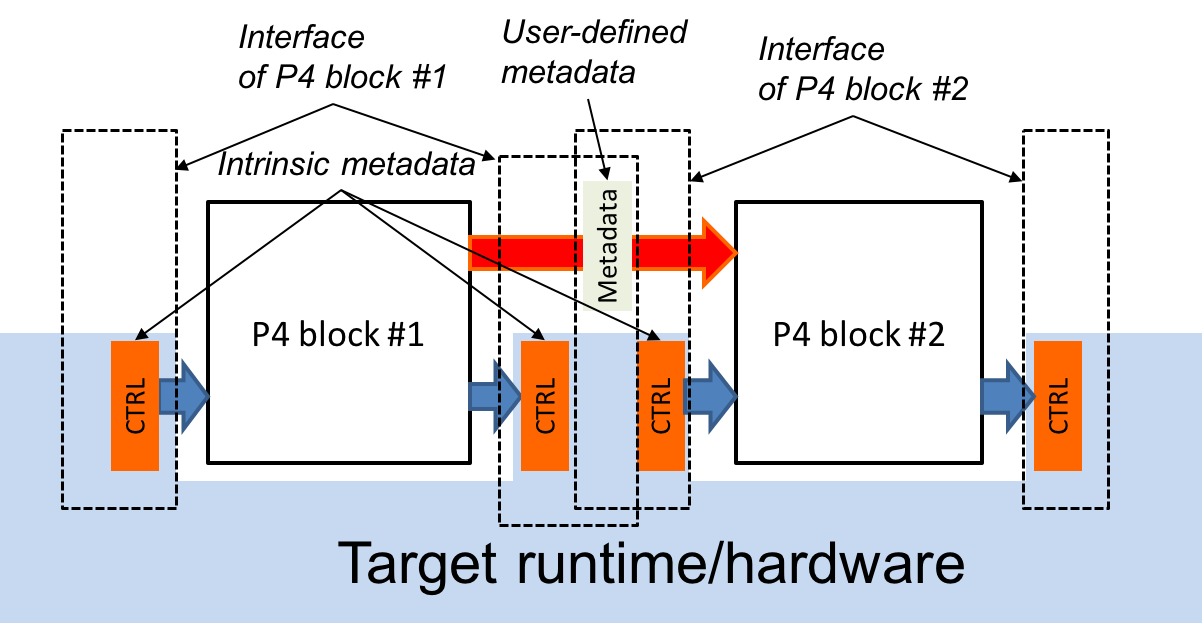
\includegraphics[width=1.00\textwidth]{resources/p4_16-architecture-model.png}

	\caption{\pfs program interfaces for an abstract architecture with two
	programmable blocks\cite{p416:v123:spec}.}
	\label{fig:arch-model}
\end{figure}

\acrshort{p4} is not a programming language for von Neumann architectures. The
abstract model assumes the target machine to be some sort of network processor
with programmable blocks embedded in a static pipeline.
Figure~\ref{fig:arch-model} illustrates such a machine and highlights the
interfaces of the \acrshort{p4} program.

A \acrshort{p4} program specifies a mapping of vectors of bits -- a bit\-vector
endomorphism. Every \acrshort{p4} program terminates; the language has no
looping constructs, a compiler can thus determine the precise maximum runtime of
a program statically.

\todo[inline]{in discussing the subpar nature of the spec, include examples of
	mistakes.
	\href{https://p4.org/p4-spec/docs/P4-16-v-1.2.3.html\#sec-minsizeinbits}{compile-time
	size determination} mentions ``\emph{Each of these method calls evaluate to
	compile-time known values that return the minimum size in bits required to
	store the expression,}'' clearly forgetting to take the \texttt{maxSize*}
	functions into account}

\subsection{Syntax}

\pfs syntax is reminiscent of imperative programming languages in the C family.
It uses prefix notation for typed bindings, braces for lexical scoping blocks,
and semicolons to separate statements. Expression syntax borrows heavily from C.

\subsection{Semantics}

The semantics of \pfs is defined in terms of abstract machines executing
imperative code. Unfortunately, the specification gives no formal treatment of
these machines; they are described only in natural language and pseudocode.

\todo[inline]{point out how the language tries to avoid undefined behaviour
and makes arithmetic typing rules saner and safer with no undef. behaviour}


%--------------------------------------%
\chapter{Language Server Architecture}
%--------------------------------------%

Language servers have a lot in common with compilers. Like compilers, they have
to build up a semantic model of a program and provide useful diagnostics for
invalid or suspicious input along the way. Unlike a compiler, a language server
needs to maintain the semantic model over the course of an editing session.
Rather than operating in batch mode, a language server runs continuously and is
expected to provide feedback within milliseconds.

However, language servers need neither to produce compilation artifacts nor to
optimise the programs they process. Instead, they are effectively
special-purpose query engines. Their output is a data structure optimised for
fast querying, such as finding references, definitions, or providing
context-sensitive completion suggestions. From that point of view, it could seem
like a language server is merely a compiler frontend\todo{decide on \& unify
"frontend" vs "front-end" (back, mid, \dots)} with very little backend logic.
Unfortunately, this is not the case.

The requirement for real-time feedback to the developer is the primary
constraint on a language server's design. For all but the most basic languages
and features, instant feedback requires an incremental computation approach and
management of state that persists across updates to source files. The second
most important consideration, and one to a large extent not shared with
compilers, is resilience to errors. While a compiler generally expects
well-formed input, a language server deals with all sorts of intermediate states
of a document, including files with many syntactic errors, invalid encodings, or
unsaved buffers outside the filesystem.

To make matters worse, while compiler frontend implementations are often guided
by a language specification\footnote{Even if, usually, an informal one.}, the
space of invalid programs is unconstrained. Developers of language servers have
to guess what intermediate states a program goes through during development and
how to respond to them. Generating meaningful semantic models from invalid input
is a challenging task, but doing so is often crucial for developers. For
example, smart auto-completion in statically typed languages is expected to
provide type-correct suggestions, even as the document being edited is
type-incorrect, and often semantically or even syntactically invalid.

In this chapter, we explore the status quo of language servers, how they differ
from conventional batch-processing compilers, how this gap may narrow in the
future, and what makes interactive language tooling difficult.

%----------------------------------------%
\section{The fruits of semantic support}
%----------------------------------------%

\todo[inline]{
	should cover LSP ``language features'' section, current tooling, show
	especially limitations of current tools with invalid input, guessing,
	complex situations (rust-analyzer failing to infer types rustc knows about),
	etc
}

The largest language servers conforming to \acrshort{lsp} offer a wide variety
of features. The vast majority of the \acrshort{api} surface is optional,
however. Upon establishing a connection, the client and server exchange
information about their respective capabilities, establishing a subset of
\acrshort{lsp} they both support.

The functionality of \acrshort{lsp} comes in two main flavours: code
comprehension and coding features. The former subsumes utilities which ease
reading and navigating through code, such as Hover (where the editor displays
details about an object under the pointer), Go to Definition, Find References,
etc. Utilities like diagnostics, auto-completion, or code actions are more
relevant to the programmer at the time they are authoring code and belong in the
latter category.

Next, we will delve into both categories and take a closer look at what they
offer.


\subsection{Code comprehension in \acrshort{lsp}}

\todo[inline]{this is lsp 3.17}

\newcommand{\org}{\pdftooltip{(original)}{This request was present in the
original LSP specification.}}

Code comprehension functionality takes up the majority of \acrshort{lsp}'s
\acrshort{api} surface and has been growing during the protocol's evolution. The
central features, already present in the initial specification of the protocol,
are Go to Definition, Find References, Document Highlight, Document Link, Hover,
Code Lens, and Document Symbols\todo{examples for everything, including a
screenshot from Neovim or something that's not VS Code. Don't forget to add
Haskell evaluation code lenses.}.

\begin{figure}[h]
	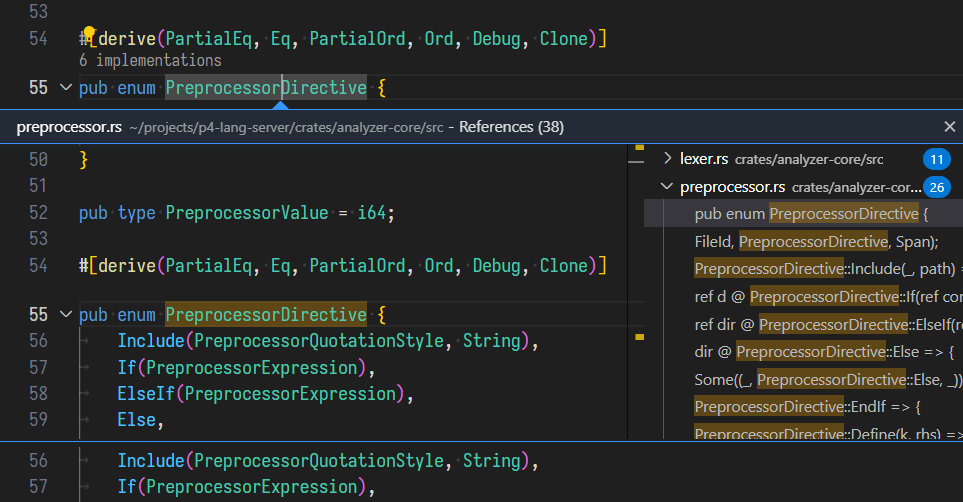
\includegraphics[width=1.00\textwidth]{resources/code_find_references.png}
	\caption{Find References in Visual Studio Code via rust-analyzer.}
\end{figure}

Go to Definition and Find References are
present in some of the oldest code comprehension tools, dating back at least to
the Unix utility \texttt{ctags}\cite{exuberant_ctags}. These let the editor jump
from a symbol's use-site to its definition and vice versa, just as their names
imply. \acrshort{lsp}'s Document Highlight request does not provide syntax
highlighting, rather, it serves to visually assist the programmer with locating
references of a given symbol without having to explicitly invoke the Find
References feature. Document Highlight could be merged with Find References
functionality, but the \acrshort{lsp} maintainers choose to keep them separate
and allow Document Highlight to report imprecise (``fuzzy'') matches. A response
to the Document Link request lists the hyperlinks embedded in the document.
Document Symbols provides a potentially hierarchical overview of the symbols of
a document, which serves the ``outline'' feature of modern editors: a tree
overview of a program's constructs, such as modules, classes, fields, and
methods. The Hover feature provides additional contextual information when
navigating code. It is typically implemented by the client rendering a pop-up
box of documentation for a given symbol. Finally, Code Lens is a versatile
editor feature for displaying additional information at a given position in a
document, such as the number of references of a type or the code metrics of a
procedure\cite{codelens_comparison}. It can trigger an action when activated,
which is used by some servers to run tests or open a Find References dialog.

\begin{figure}[t]\centering
	\begin{multicols}{2}
	\begin{enumerate}
		\item Go to Declaration
		\item Go to Definition \org
		\item Go to Type Definition
		\item Go to Implementation
		\item Find References \org
		\item Prepare Call Hierarchy
		\item Call Hierarchy Incoming Calls
		\item Call Hierarchy Outgoing Calls
		\item Prepare Type Hierarchy
		\item Type Hierarchy Super Types
		\item Type Hierarchy Sub Types
		\item Document Highlight \org
		\item Document Link \org
		\item Document Link Resolve \org
		\item Hover \org
		\item Code Lens \org
		\item Code Lens Refresh
		\item Folding Range
		\item Selection Range
		\item Document Symbols \org
		\item Semantic Tokens
		\item Inlay Hint
		\item Inlay Hint Resolve
		\item Inlay Hint Refresh
		\item Document Color
	\end{enumerate}
	\end{multicols}

	\caption{Code comprehension -related requests in \acrshort{lsp} 3.17.}
	\label{fig:comprehension-requests}
\end{figure}


\subsection{Coding features in \acrshort{lsp}}

A shorter but no less important range of \acrshort{api} calls supports the
developer right when they are authoring code. The main features are
auto-completion, signature help, formatting, and symbol renaming.

\begin{figure}
	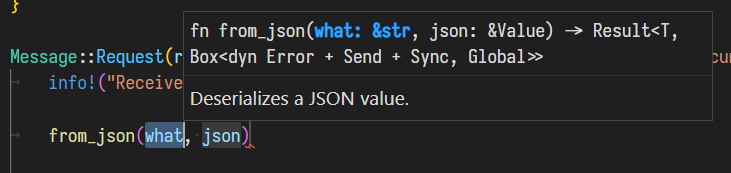
\includegraphics[width=1.00\textwidth]{resources/code_signature_help.png}
	\caption{Signature help in VS Code for Rust shows a pop-up with
	documentation as well as the signature of the callee, highlighting the
	parameter under cursor.}
\end{figure}

Auto-completion offers to fill in code as the programmer is typing, supports
ranking results based on their relevance, on both the server and the client
side, and can include a ``quick info'' description for each option. Signature
help shows parameter name and type information when calling a procedure, method,
or function. Formatting allows a language server to rewrite a document upon
request, for example to conform to a particular code style. The \acrshort{lsp}
formatting functionality can format either the entire document, a selected
range, or reactively an arbitrary part of the document as the user types.
Finally, symbol renaming performs a context-sensitive workspace-wide rename of a
given symbol.

\begin{figure}[t]\centering
	\begin{multicols}{3}
	\begin{enumerate}
		\item Inline Value
		\item Inline Value Refresh
		\item Moniker
		\item Completion Proposals \org
		\item Completion Item Resolve \org
		\item Publish Diagnostics
		\item Pull Diagnostics
		\item Signature Help \org
		\item Code Action
		\item Code Action Resolve
		\item Color Presentation
		\item Formatting \org
		\item Range Formatting \org
		\item On type Formatting \org
		\item Rename \org
		\item Prepare Rename
		\item Linked Editing Range
	\end{enumerate}
	\end{multicols}

	\caption{Coding language features in \acrshort{lsp} 3.17.}
	\label{fig:coding-requests}
\end{figure}

Later \acrshort{lsp} revisions added high-level features not universally
applicable to all programming languages. For instance, version 3.16 added
\emph{linked editing}, which some conforming implementations use to update
opening and closing \acrshort{xml} tags seamlessly without the user specifically
triggering a rename action. Version 3.17 introduced \emph{type hierarchy}
requests, relevant only to programming languages with subtyping. On the other
hand, more general facets of the protocol see creative use in unintended
contexts. One example is the use of lenses and special comments in the Haskell
Language Server project\cite{haskell_ls} to provide \acrshort{repl}-like
functionality. Another is the LT$_\text{E}$X Visual Studio Code
extension\cite{vscode_spellcheck}, which provides spell and grammar checking in
Markdown and \LaTeX~documents, as well as in programming language comments. Even
though \acrshort{lsp} has no built-in support for extracting the comments of a
document or for spell checking in general, LT$_\text{E}$X achieves this with a
combination of non-\acrshort{lsp} \acrshort{api}s and by leveraging
\acrshort{lsp} diagnostics and code actions to provide suggested spellings.

\begin{figure}[h]\centering
	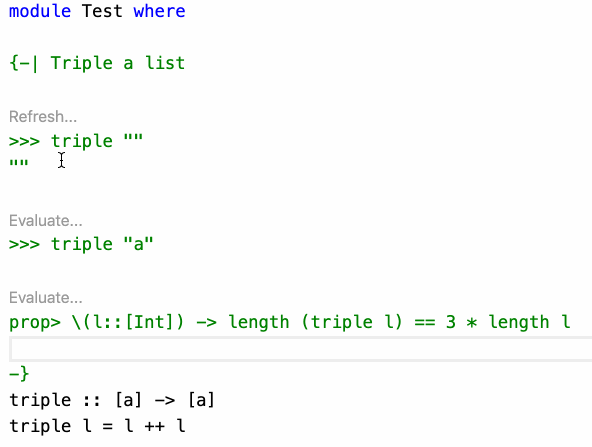
\includegraphics[height=0.3\textheight]{resources/code_haskell_repl.png}
	\caption{The Haskell Language Server project supports in-editor expression
	evaluation in comments prefixed with \texttt{>>>} and checking QuickCheck
	properties in comments starting with \texttt{prop>}.}
\end{figure}

\subsection{The state of the art}

Some of the best tooling in the \acrshort{lsp} ecosystem comes, somewhat
unsurprisingly, from Microsoft.

Projects which served as the de facto \acrshort{ide} integration for the given
language matured somewhat quicker than software that already had ample
competition.

\todo[inline]{the idea here is to compare "actual" language popularity
with the popularity of a corresponding language server.
We should see people preferring other tools for established technologies.}

We have chosen to exclude some technologies from this comparison. JavaScript,
TypeScript, CSS, and HTML support is built into VS Code and therefore does not
show up in VS Code marketplace statistics for installed language extensions.
SQL, while popular, has too many dialects to present a faithful picture through
the lens of extension installations alone. These technologies were in turn
filtered out from StackOverflow's list of most popular languages to highlight
the differences in ranking.

\todo[inline]{
	add the source
	% https://marketplace.visualstudio.com/search?target=VSCode&category=Programming%20Languages&sortBy=Installs
}

\begin{table}\centering
\caption{Popularity of programming languages among VS Code users and
StackOverflow's 2022 Developer survey\cite{stackoverflow_survey_2022}
respondents.}
\begin{tabular}{|r|c|c|}
	Rank & VS Code extension & Most popular programming and scripting languages
	\tabularnewline \hline
	1  & Python     & Python     \tabularnewline
	2  & C/C++      & Java       \tabularnewline
	3  & Java       & C\#        \tabularnewline
	4  & C\#        & C/C++      \tabularnewline
	5  & Go         & PHP        \tabularnewline
	6  & PHP        & PowerShell \tabularnewline
	7  & PowerShell & Go         \tabularnewline
	8  & Dart       & Rust       \tabularnewline
	9  & Ruby       & Dart       \tabularnewline
	10 & Rust       & Ruby       \tabularnewline
\end{tabular}
\end{table}



%---------------%
\chapter{Design}
%---------------%

\todo[inline]{the design of the p4 language server, what it learned from
rust-analyzer, etc}

\begin{itemize}
	\item intention to do everything in-editor, Rust to WebAssembly
	\item cannot reuse the open-source frontend, not error-tolerant, difficult
	to work with, poor diagnostics
	\item needs to adapt to various backends and architectures easily
	\item open-source project, no point in keeping it closed, want to encourage
	contributions from the community
\end{itemize}

The high-level architecture of the \acrshort{p4} Analyzer project marks a
departure from conventional language server designs in that it primarily targets
WebAssembly and aims to run entirely within the Visual Studio Code editor. This
decision makes installation simpler for the end-user, cross-platform support
easier for the developers, and security policy conformance trivial for any
security teams involved.

The main mode of operation is thus as follows: the language server runs in a
WebAssembly worker of the \acrshort{p4} Analyzer VS Code extension. The
extension itself defines a simple TextMate\todo{reference} grammar specification
and serves as a thin client for the server. The main bulk of \acrshort{lsp}
functionality is delegated to the editor. VS Code forwards edits to open files
to the language server, which updates its model of the workspace. When VS Code
asks for completions, hover, diagnostics, or other features, the analyzer
recomputes necessary information on-demand and responds appropriately.

In addition to the WebAssembly executable, the \acrshort{p4} Analyzer project
also compiles to a native binary that executes in a standalone process and
communicates with an arbitrary \acrshort{lsp}-compliant client over a socket.
However, the standalone language server requires support for certain features
related to filesystem functionality that fall outside the protocol
specification. We will discuss these in-depth later\todo{make sure this is
indeed the case, put a reference here}.

%--------------------------------------------%
\section{The \acrshort{p4} Analyzer pipeline}
%--------------------------------------------%

The first step in our pipeline is lexical analysis. Somewhat unconventionally,
our lexer produces tokens even for the preprocessor (i.e. it analyses
preprocessor directives). Our preprocessor then operates at the lexeme level,
rather than running separately as the first step. This requires a
reimplementation of the preprocessor, which is already necessitated by
fault-tolerance and WebAssembly support requirements anyway. On the upside, a
custom preprocessor simplifies tracking of source positions, which are crucial
for accurate diagnostics.

\subsection{Lexical analysis}

The \pfs specification defines a \acrshort{yacc}\todo{use a glossary entry
instead of an acronym}/Bison grammar for the language. However, this grammar has
several flaws.

The primary issue is that it does not maintain a clean separation between a
parser and a lexer and requires these two components to collaborate.

\begin{displayquote}
	\textit{The grammar is actually ambiguous, so the lexer and the parser must
	collaborate for parsing the language. In particular, the lexer must be able
	to distinguish two kinds of identifiers:}

	\begin{itemize}
		\item \textit{Type names previously introduced (\texttt{TYPE\_IDENTIFIER}
		tokens)}
		\item \textit{Regular identifiers (\texttt{IDENTIFIER} token)}
	\end{itemize}

	\textit{The parser has to use a symbol table to indicate to the lexer how to
	parse subsequent appearances of identifiers.}

	-- \citetitle{p416:v123:spec} \cite{p416:v123:spec}
\end{displayquote}

The specification goes on to show an example where the lexer output depends on
the parser state and mentions that the presented grammar ``\textit{has been heavily
influenced by limitations of the Bison parser generator tool.}''

The tight coupling between the lexer and the parser, as well as the decision to
remain in the confines of an outdated parser generator despite its many
drawbacks, are in our opinion examples of poor design for a language born in the
twenty-first century. We have elected not to follow this ambiguous grammar
specification in the \acrshort{p4} Analyzer project and instead build a pipeline
that is tolerant to invalid input to the fullest extent possible, while
accepting the same language.

Our lexer's task is to convert the input string into a stream of lexemes. The
lexer is a standalone finite state machine independent of any later stages in
the pipeline. It has a secondary output for reporting diagnostics, but this side
channel is write-only.

\subsubsection*{Error tolerance}

Error tolerance at the lexer level means proceeding with lexeme stream
generation despite nonsensical input. We emit a special error token whenever
such input is encountered. Additionally, the lexer validates numeric constants,
which can specify width, base, and signedness\todo{is this a word?}. These
properties could be out of bounds for a given literal. In these cases, the lexer
produces\todo{"should produce" language instead? since this is a design chapter,
wink wink?} a valid token anyway but logs an error-level diagnostic, which is
reported to the user once lexing completes.


\subsection{The preprocessor}

\pfs requires support for a preprocessor, very similar to the C preprocessor,
directly in the specification. However, it does not ask implementors to support
the entirety of \texttt{cpp}. Notably, only simple, parameter-less macros are
allowed. This is already enough to necessitate running the preprocessor before
starting the parser, however. Consider the code in
Listing~\ref{lst:p4pp}\todo{p4 syntax would be nice}. These examples show how
grammatically invalid code may become valid and vice versa, based only on the
right-hand sides of preprocessor macros.

An important consideration for a correct implementation of preprocessor
directives is their context-sensitive nature. Expressions for conditional
inclusion in directives \texttt{\#if}, \texttt{\#elif}, and \texttt{\#ifdef} are
themselves subject to macro substitution and thus have to be kept in plain text
or lexeme form until their evaluation.

One more thing to note here is the mechanism of document inclusion. Before
analysing a \pfs source file (at least to some degree), the full extent of its
dependencies is unknown and arbitrary. The language has no module system and
imposes no restriction on the paths a source file can include. This poses a
challenge for lexeme-level preprocessors, as a file needs to be lexed before it
can be included. To deal with this, a correct implementation should collect the
paths a source file can depend on, lex their contents, and include their lexemes
in the preprocessed lexeme stream. This is of particular note in our
implementation, as the collection of dependencies reports this dependency set to
the editor to set up filesystem-level watches. Subsequent edits to the
dependencies, or even to the dependency set itself, can be processed
incrementally.

\subsubsection*{Error tolerance}

Error tolerance in the preprocessor means reporting errors and warnings about
malformed input to the user while continuing to interpret directives in the
input stream on a best-effort basis. Mistakes in preprocessor directives come in
several flavours.

The directive itself may be malformed, either due to a typo in its name or a
problem in some of its arguments. The former case will simply be lexed as an
unrecognized directive and reported as such. It is possible to suggest fixes for
common typos to the user. A problem in the directive's argument or arguments
needs to be resolved based on its meaning. For example, an \texttt{\#include}
directive could point to a non-existent file, the preprocessor should then
report this error and proceed as if the file were not included. This is likely
to lead to further errors down the road, but without knowledge of the referenced
file's contents, it is the best a preprocessor can do.

Another class of errors is semantic and context-sensitive in nature: a directive
may be used in the incorrect context or missing where it is expected. For
example, a user may forget to add an \texttt{\#endif} directive, or include more
than one \texttt{\#else} directive for a condition. Unfortunately, guessing the
user's intention when faced with any syntactic or semantic problems in the input
is a tall order. No guarantees of optimality can be given, as is often the case
with similar heuristics. In the duplicate \texttt{\#else} problem, the
preprocessor could be reasonably expected to either skip over the first
\texttt{\#else}'s body, the second \texttt{\#else}'s body, or assume either of
the directives was inserted by accident and pretend it is not a part of the
input stream. We choose to skip the second \texttt{\#else}'s body in our design,
but other strategies are equally valid\todo{maybe it'd be better to look at some
data from users. But does this matter enough to bother with a study?}.

\begin{lstlisting}[
	caption={~\pfs preprocessor example},
	label=lst:p4pp,
	captionpos=t,
	tabsize=4,
	float,
	abovecaptionskip=-\medskipamount,
	belowcaptionskip=\medskipamount,
	language=c
]
#define op +
// #define op 2

#define paren )

header h {
	bit<1> field;
}

control pipe(inout h hdr) {
	Checksum16() ck;
	apply {
		// arithmetic expression could be invalid
		h.field = 1 op 3;
		// a parse without prior macro substitution would fail
		ck.clear( paren;
		// this would parse correctly, but macro substitution
		// will reveal a parse error
		ck.update(op);
	}
}
\end{lstlisting}


\subsection{The parser}

The next natural step in the pipeline is the act of finding the productions of a
\pfs grammar that match the preprocessed input program; parsing. While the steps
up to this point are fairly simplistic and efficient, parsing is a
resource-intensive process. A language server is expected to provide real-time
feedback to the developer, including auto-completion suggestions updated with
every keypress\todo{the lexer can identify a caret inside a (possibly
unfinished!) comment or string. Maybe we can learn from that for naive
lexer-based auto-completion?}. Low latency is crucial to the end-user and the
parser lies on every critical path from user input to high-level results shown
in the editor's interface. At the same time, a typical \pfs program is likely to
consist of a long prefix that does not change between edits and a
user-maintained suffix that changes frequently. This is because a \pfs program
usually begins with \texttt{\#include} directives referencing platform-specific
files with constants, error codes, \texttt{extern} definitions and other shared
code. These constraints and ???\todo{word here} are a very good fit for the
field of \emph{incremental parsing}.

An incremental parser aims to reuse previously computed information about the
input in response to small perturbations. Our parser specifically builds on
incremental packrat parsing\cite{dubroy2017incremental_packrat_parsing}, which
places few constraints on grammar design and is easy to implement in an
extensible manner.


\subsubsection*{Error tolerance}

Error tolerance in parsing is far more nuanced than in any of the previous
steps, which is not surprising with regard to the relative complexity of the
languages the individual steps recognize and process.


% 3 new pages: LuaJIT-friendly sort
% 5 new pages: look into CC playback
% 7 new pages: build the game world, including saves

\listoftodos[Work in progress]
 % include `text.tex' from `text/' subdirectory

\appendix\appendixinit % do not remove these two commands

\chapter{Nějaká příloha}


Sem přijde to, co nepatří do hlavní části.
 % include `appendix.tex' from `text/' subdirectory

\backmatter % do not remove this command

\printbibliography % print out the BibLaTeX-generated bibliography list

\chapter{Obsah přiloženého média}


	\dirtree{%
		.1 readme.txt\DTcomment{stručný popis obsahu média}.
		.1 exe\DTcomment{adresář se spustitelnou formou implementace}.
		.1 src.
		.2 impl\DTcomment{zdrojové kódy implementace}.
		.2 thesis\DTcomment{zdrojová forma práce ve formátu \LaTeX{}}.
		.1 text\DTcomment{text práce}.
		.2 thesis.pdf\DTcomment{text práce ve formátu PDF}.
	}
 % include `medium.tex' from `text/' subdirectory

\end{document}
